%% This is an example first chapter.  You should put chapter/appendix that you
%% write into a separate file, and add a line \include{yourfilename} to
%% main.tex, where `yourfilename.tex' is the name of the chapter/appendix file.
%% You can process specific files by typing their names in at the 
%% \files=
%% prompt when you run the file main.tex through LaTeX.
\chapter{Generative Adversarial Networks for Market Data Generation}

\section{Overview of Generative Adversarial Networks}
\subsection{Vanilla GAN (VGAN)}
Generative adversarial networks (GANs) are one type of powerful generative AI that serve as the backbone of many applications in synthetic data generation and recent Deepfake technology. GANs were first introduced as an innovative unsupervised framework to generate synthetic data that represents real data by simultaneously training a generator and discriminator to learn the underlying distribution of the real data. Ian J. Goodfellow et al. (2014) demonstrated the efficacy of GANs in generating synthetic data that resemble the properties of real data \cite{gans}. The generator takes real input data $x$ and adds Gaussian-distributed random noise $z$ to output synthetic data, while the discriminator tries to distinguish the output from the generator and the real data. As the discriminator performs better in distinguishing real and synthetic data, the generator learns more about the underlying distribution and becomes better at generating new data. Vanilla GANs (VGAN) have been very successful in generating fake images and videos. During the training process, the discriminator acts as a classifier and outputs a probability that the generator-produced sample is fake. The standard machine learning process of using gradient descent is performed to continuously improve both the generator and discriminator simultaneously. The objective function of the generator $G$ and discriminator $D$ used to update the GAN's weights, computed at each training iteration, is given by the following value function $V$ in which the generator tries to minimize and the discriminator tries to maximize.
\begin{equation}
    \min_{G}\max_{D}V(D,G) = E_{x\sim p_{data}(x)}[\log{D(x)}]+E_{z\sim p_{z}(z)}[\log(1-D(G(z)))]
\end{equation}
In the context of generating market data, real historical time-series data of equity markets are used as input instead of images. The end goal is still the same, which is to produce representative synthetic data that exhibit similar properties as the real data. The structure of a vanilla GAN is displayed in Figure 2-1.
\begin{figure}[H]
\centering
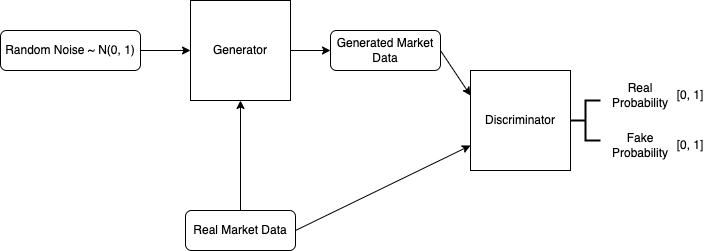
\includegraphics[width=15cm]{templates/assets/gan/gan_architecture.png}
\caption{Structure of a Vanilla GAN}
\end{figure}
\noindent The generator and discriminator compete in a zero-sum game with the objective of training the generator to outperform the discriminator. At each training iteration, the loss is computed given the discriminator's performance and the errors are backpropagated through the generator and discriminator to adjust weights. As the discriminator becomes better at distinguishing real and fake data, the generator has a higher loss and is forced to adjust its weights to generate data that follow the distribution of real data more closely. At the end of the training process, the generator is able to produce new data that resembles the original data, since it has learned the distribution of the real data during the training process.

\subsubsection{Applications of GANs}
GANs have mostly been used for image processing tasks such as generating fake images or performing adversarial attacks on neural networks. However, the framework of GANs can be extended to work with other types of data as well, including tabular and time-series data. This has great implications for working with financial data, as the majority of data in finance consists of tabular and time-series data, such as asset price movement and limit order books. Similar to the GANs used in Deepfake technology, GANs also have the potential to learn the underlying distributions and data-generating processes of price evolution and order books. This allows GANs to learn the market microstructure and price evolution process directly from data instead of relying on various parametric assumptions about market dynamics.

\subsection{Wasserstein GAN (WGAN)}
Nevertheless, vanilla GANs often suffer from a common problem known as mode collapse, where the model hits a local minimum during the training process and is unable to continue learning from the data. Very often, this issue arises with the structure of the GAN due to the non-convexity of the discriminator's loss function during training. Mode collapse ultimately results in the generator producing the same data with the discriminator unable to learn to distinguish this fake. For example, if the generator learns to produce one possible path of simulated market data that is indistinguishable from real market data to the discriminator, then the generator will continue producing this single instance of market data. This can be caused by a variety of factors, with vanishing gradients in the discriminator as one possibility. In order to implement a useful market simulator, the generator component of the GAN must be versatile and learn to generate a large variety of synthetic data that is representative of empirical data. To achieve this versatility, it is essential that the discriminator can perform well during the training process to force the generator to learn to generate a diverse set of useful representations of market data.
\\
\\
Many alternative forms of GANs have been proposed to tackle this issue. One method to address the issue of mode collapse in vanilla GANs is to adjust the output of the discriminator so that it returns a score instead of a probability. Rather than being strictly a classifier of real and fake images, it is possible to turn the discriminator into a critic of generated data instead. This creates the benefit of allowing the discriminator output to exceed the bound of 0 to 1, which can alleviate the effects of vanishing gradients and mode collapse. Arjovsky, Chintala, and Bottou (2017) explore the use of Wasserstein GANs (WGAN) \cite{wgan} to implement this idea by using the Wasserstein loss metric as the output of the discriminator. We will not delve into the derivation of gradient descent, but instead, focus on the implementation with financial data. With a set of 1-Lipschitz functions $D_f$, the Wasserstein GAN value function is defined by:
\begin{equation}
    \min_{G}\max_{D}V_W(D,G) = E_{x\sim p_{data}(x)}[D_f(x)]+E_{z\sim p_{z}(z)}[D_f(G(z))]
\end{equation}
\noindent Instead of making classifications like the discriminator of a VGAN does, the discriminator of a WGAN computes the Wasserstein distance and uses this loss to update weights. The other components of the model remain relatively similar. The structure of a Wasserstein GAN is displayed in Figure 2-2.
\begin{figure}[H]
\centering
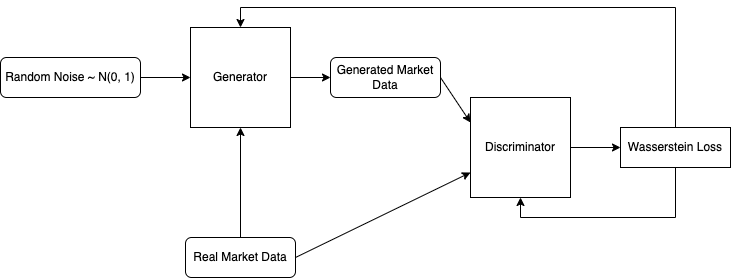
\includegraphics[width=15cm]{templates/assets/gan/wgan_architecture.png}
\caption{Structure of a Wasserstein GAN}
\end{figure}
\noindent For implementing a useful synthetic market environment, the generator must be robust in creating market data from a wide range of possible market conditions and possibilities. Gulrajani et al. (2017) propose an additional improvement to the original WGAN framework by introducing a critic gradient penalty \cite{wgan-gp} instead of the standard weight clipping approach in the training process, which will further help with mitigating mode collapse and promoting stability in data generation. The gradient penalty, combined with the use of Wasserstein distance, greatly improves the GAN's ability to learn robust representations of real market data. This model can now be trained using historical financial data, and the trained generator can be used to construct a representative synthetic market environment which may be useful for a variety of applications, particularly for machine learning methods.

\subsection{Other Forms of GANs}

Additional studies have been done in devising new methods to alter the GAN's structure to improve performance in generating better data. Many other forms of GANs have recently been developed, many of which serve a specific task in data generation. For example, many GANs have been tailored to work particularly on time-series data, which exhibit properties that differ from image data. As time-series data often has high complexities, some variations of GANs are implemented using convolutional and recurrent neural networks in the generators and discriminators to learn sequential data. Olof Mogren (2016) describes Continuous Recurrent Neural Network GANs (C-RNN-GAN) \cite{crnngan}, a variation of GANs, to generate continuous sequential data. Nevertheless, the proposed framework, unlike WGANs, relies on the classification framework and may suffer from mode collapse issues when applied to financial data.

\subsubsection{Time-Series GANs}
One specific feature of time-series data that differs from other types of data is that time-series exhibit various temporal dynamics, which should be preserved when using a GAN to generate time-series data. However, the original framework of GANs does not provide any specific means of learning and maintaining temporal correlations on time series. A notable extension of the GAN framework to work with time-series data is the Time-Series GAN. Jinsung Yoon, Daniel Jarrett, and Mihaela van der Schaar (2019) discuss solutions to this problem and propose a modification of GANs to generate more-realistic time-series data that maintain statistical and temporal properties \cite{tsgan}. The Time-Series GAN (TimeGAN) preserves the temporal dynamics of time-series data by introducing a step-wise supervised loss to allow the generator and discriminator to learn the conditional distribution of the data, as well as an embedding network to reduce the dimensionality of the feature space during training. TimeGAN combines the adversarial learning framework with autoencoders to simultaneously learn and optimize the supervised and unsupervised losses, as shown below.
\begin{figure}[H]
\centering
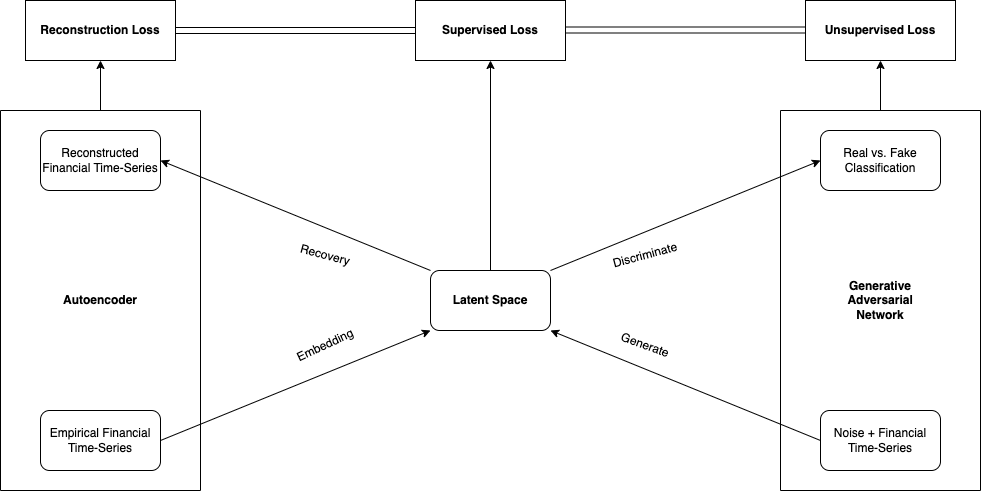
\includegraphics[width=15cm]{templates/assets/gan/tsgan_architecture.png}
\caption{Structure of a Time-Series GAN}
\end{figure}

\section{Using GANs for Synthetic Data Generation}
Although state-of-the-art applications of GANs involve image processing tasks, this framework can be adapted to work with data other than images, including tabular and time-series data. The goal of using GANs as an alternative approach to generating and simulating data is to remove the need for parameterization and assumptions about market dynamics. Since GANs are an unsupervised learning and non-parametric framework, they learn the distribution directly from real data instead of relying on the careful selection of parameters.
\\
\\
The trained generator portion of the GAN can be used to generate new data given a starting point and random noise input. During the synthetic data generation process, the discriminator portion of the GAN is not required, as it served its primary purpose of improving the generator and helping it learn the underlying data-generating process during training. As discussed before, the objective of the GAN is to generate a diverse set of possible market scenarios representative of the true patterns and dynamics observed in empirical market data. In the context of simulating financial time-series data of spot prices in the market, this translates into using the generator to generate spot price paths that have relatively similar distributional statistics and movement patterns to real spot price data \cite{stock-gan}.
\\
\\
Markets can be bullish, bearish, or stagnant at most points in time, but true market dynamics can be incredibly complex and noisy which presents a huge challenge for working with financial data. Ideally, the generator will be able to simulate many possible market scenarios that are representative of the complexity and noisiness present in empirical data. The possibilities and randomness of market dynamics are represented as random noise inputted into the generator when generating data.
\subsection{Simulating Financial Market Data with GANs}
Although the model can be adapted to work with any asset that has historical data available, we will focus on using the trained model for a specific stock, such as Apple (AAPL). AAPL has an abundance of historical price data available, dating back to the 1980s, with over 40 years of data. The generator requires a starting point in the financial time series to then input random noise and generate new data. Of course, at any point in time during the life of the company, there is a current price level and an unpredictable and uncertain future trend. Being able to simulate many realistically possible paths of data can be useful for training and evaluating algorithms that require an abundance of data. With the trained GAN, a large number of data points can be generated by simply producing random noise as input. The generator uses a starting point and combines random noise with the underlying distribution it has learned during training. Using the trained generator to simulate one path of spot prices for AAPL yields the following results displayed below.
\begin{figure}[h]
\centering
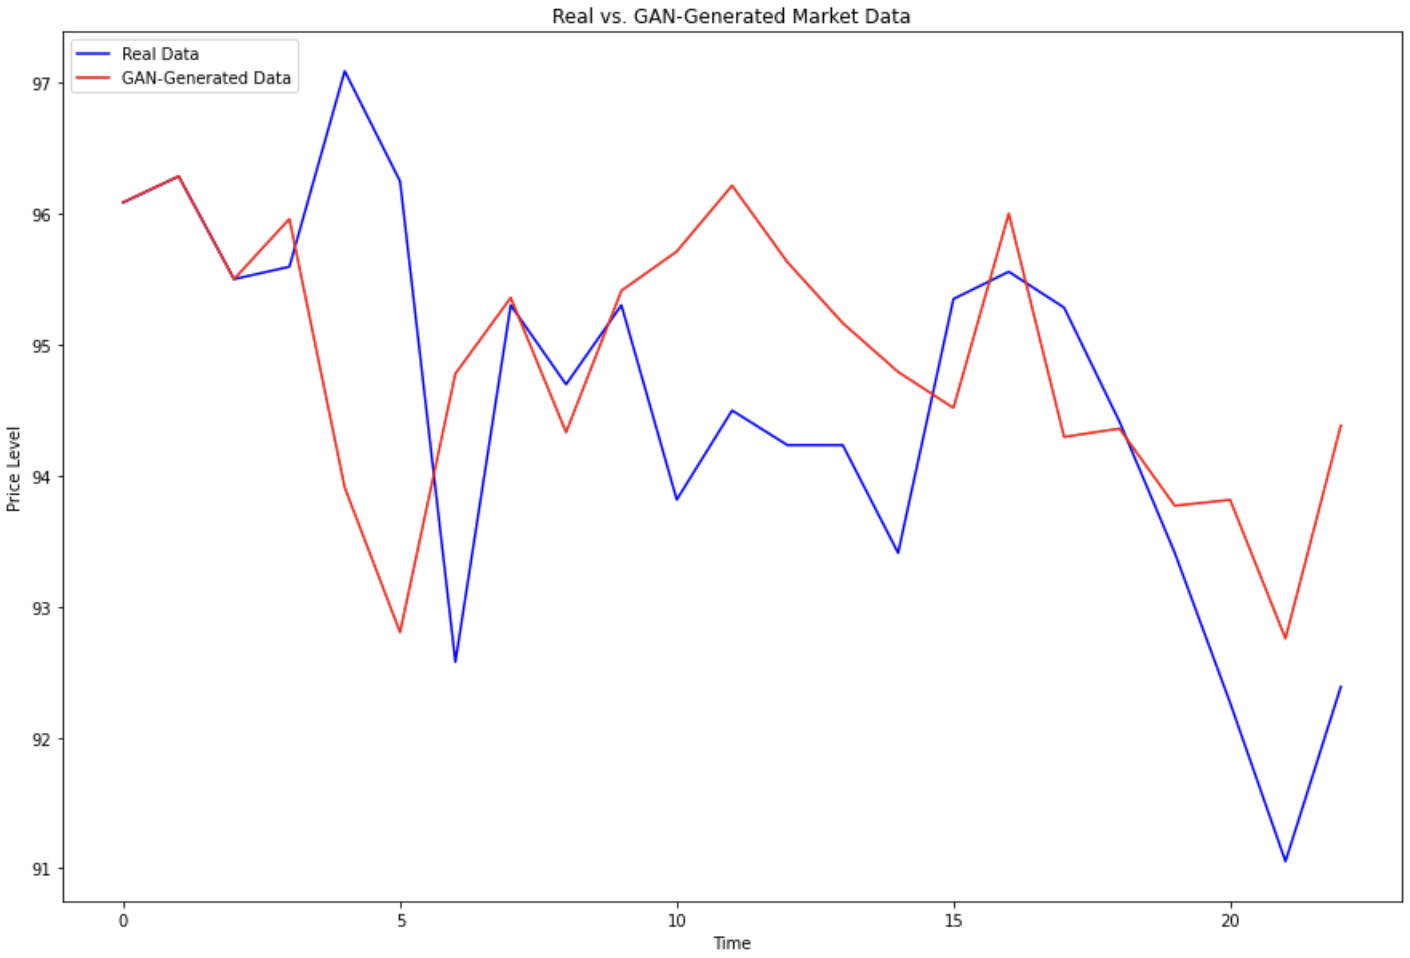
\includegraphics[width=14.5cm]{templates/assets/gan/gan_stable.png}
\caption{GAN-Based Spot Price Simulation}
\end{figure}
\\
\noindent As we can qualitatively see in the plot above, the generated data exhibits similar properties as the real data and has similar movement patterns. The real and generated data both have the same starting point, at a price level of around \$96, but the GAN has learned the dynamics of AAPL's historic price movement and has generated another plausible scenario of how the price might have evolved over time. This systematic data generation framework has great implications for a variety of financial applications, most importantly enhancing algorithms that require lots of data. The generation of many alternative paths from a starting point can be used as data to train and evaluate models and strategies. Ideally, the models and strategies that traders and investors develop are robust to different market conditions and possibilities, which can be captured by the GANs trained on historical market data.
\\ \\
For example, the generator of the GAN would ideally be able to produce a diverse set of market data, including data under both bullish and bearish markets. Using the trained generator, the diagrams below show AI-generated instances of the evolution of AAPL in bullish and bearish conditions.
\begin{figure}[h]
\centering
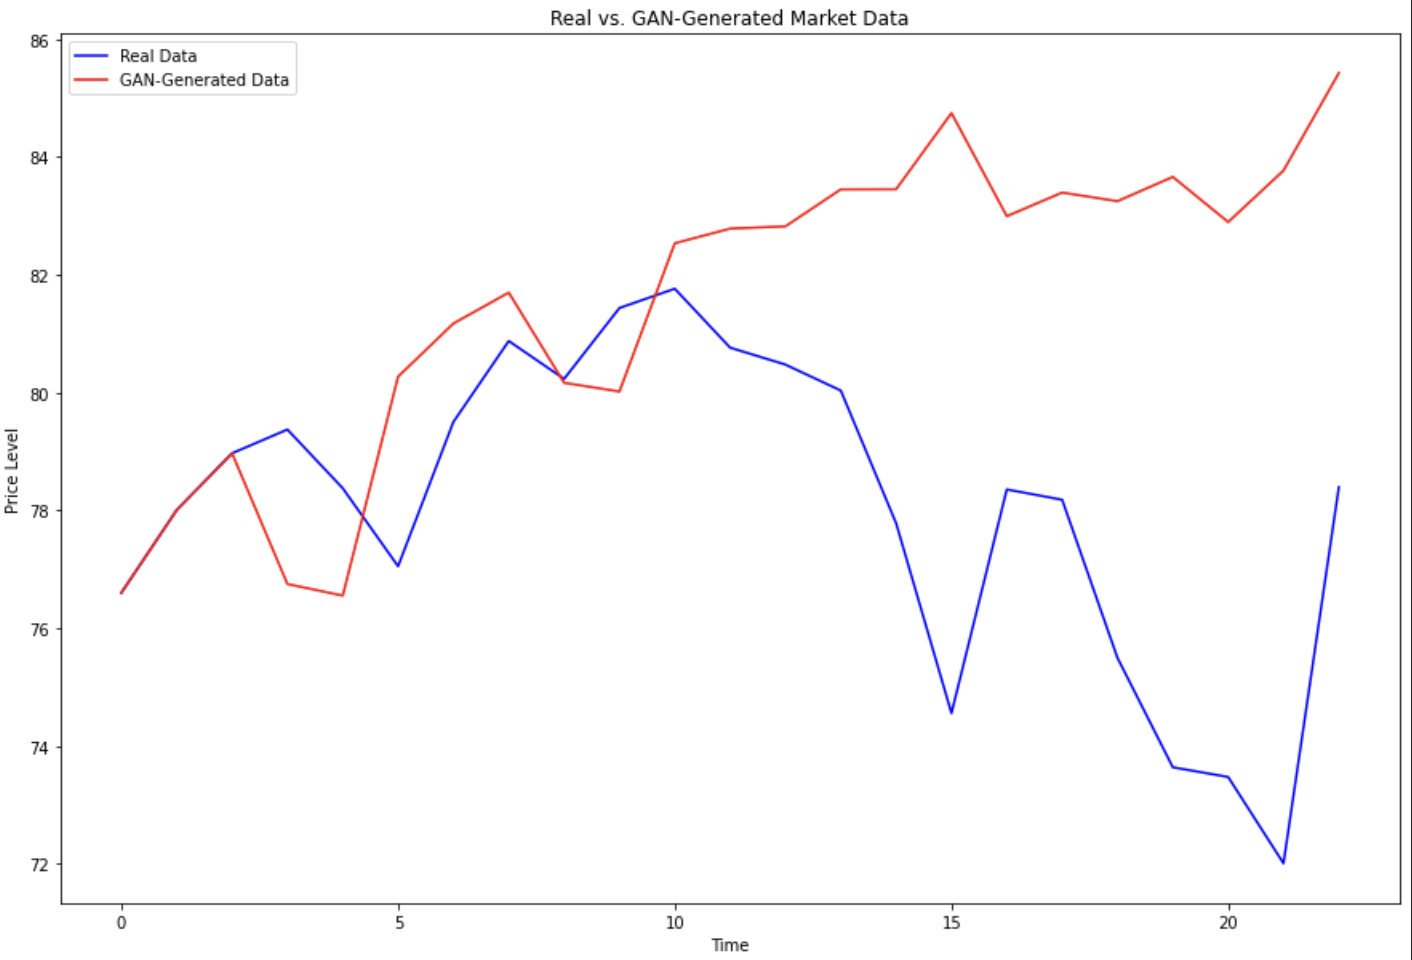
\includegraphics[width=11cm]{templates/assets/gan/gan_up.png}
\caption{Upwards Trend Path Simulated by GAN}
\end{figure}
\begin{figure}[h]
\centering
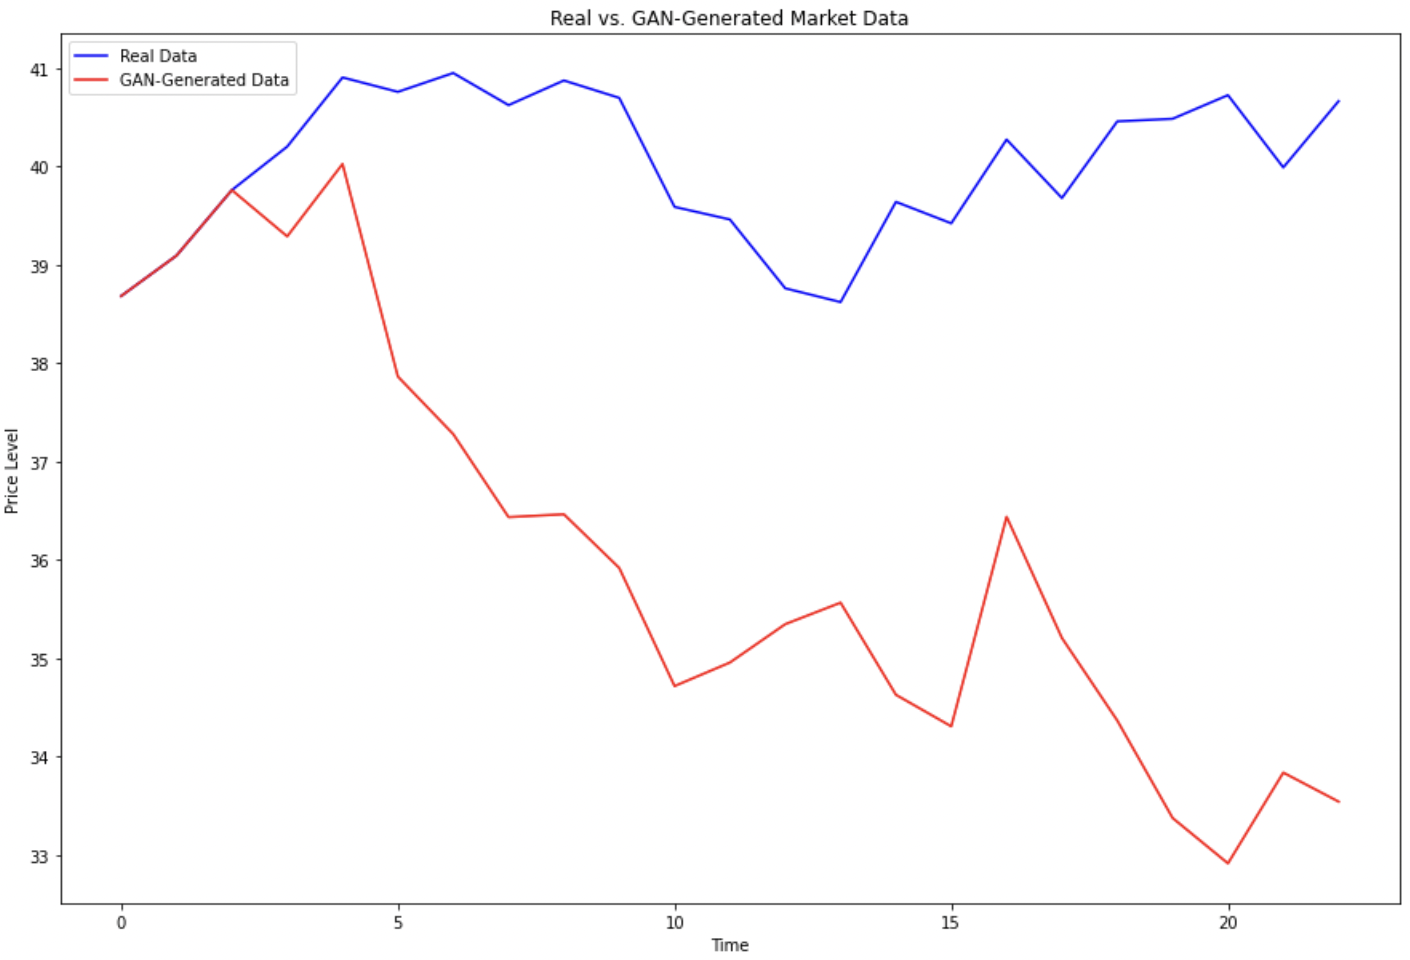
\includegraphics[width=11cm]{templates/assets/gan/gan_down.png}
\caption{Downwards Trend Path Simulated by GAN}
\end{figure}
\\
\noindent The figure above shows an AI-generated path that has an upward trend compared to the real historical data. As shown above, the red lines represent the GAN-generated data and the blue lines represent the actual data. In figure 2-5, the generated data appears to have an upward trend relative to the actual historical data, while in figure 2-6, the generated data appears to have a downward trend relative to the actual historical data. Although the real and generated data have different trends, the temporal properties of stock price dynamics appear to be relatively similar. This divergence in the real and generated paths, along with the preservation of price movement dynamics, is essential for being able to use GAN-generated data for training and evaluating models and strategies. It is possible to use this generator to generate an abundance of realistic market data under various market scenarios, similar to using Monte Carlo simulations. The difference is that while Monte Carlo simulations are parametric and probability-based, which may not capture the complexities and patterns of real market dynamics, GAN-generated data exhibits properties similar to empirical data and has a similar underlying distribution. It is interesting to observe, however, that a plot of GAN-generated series looks very similar to Monte Carlo simulations since both methods capture a variety of possibilities of stock price movement. A plot of GAN-based market simulation for AAPL is displayed below.
\begin{figure}[h]
\centering
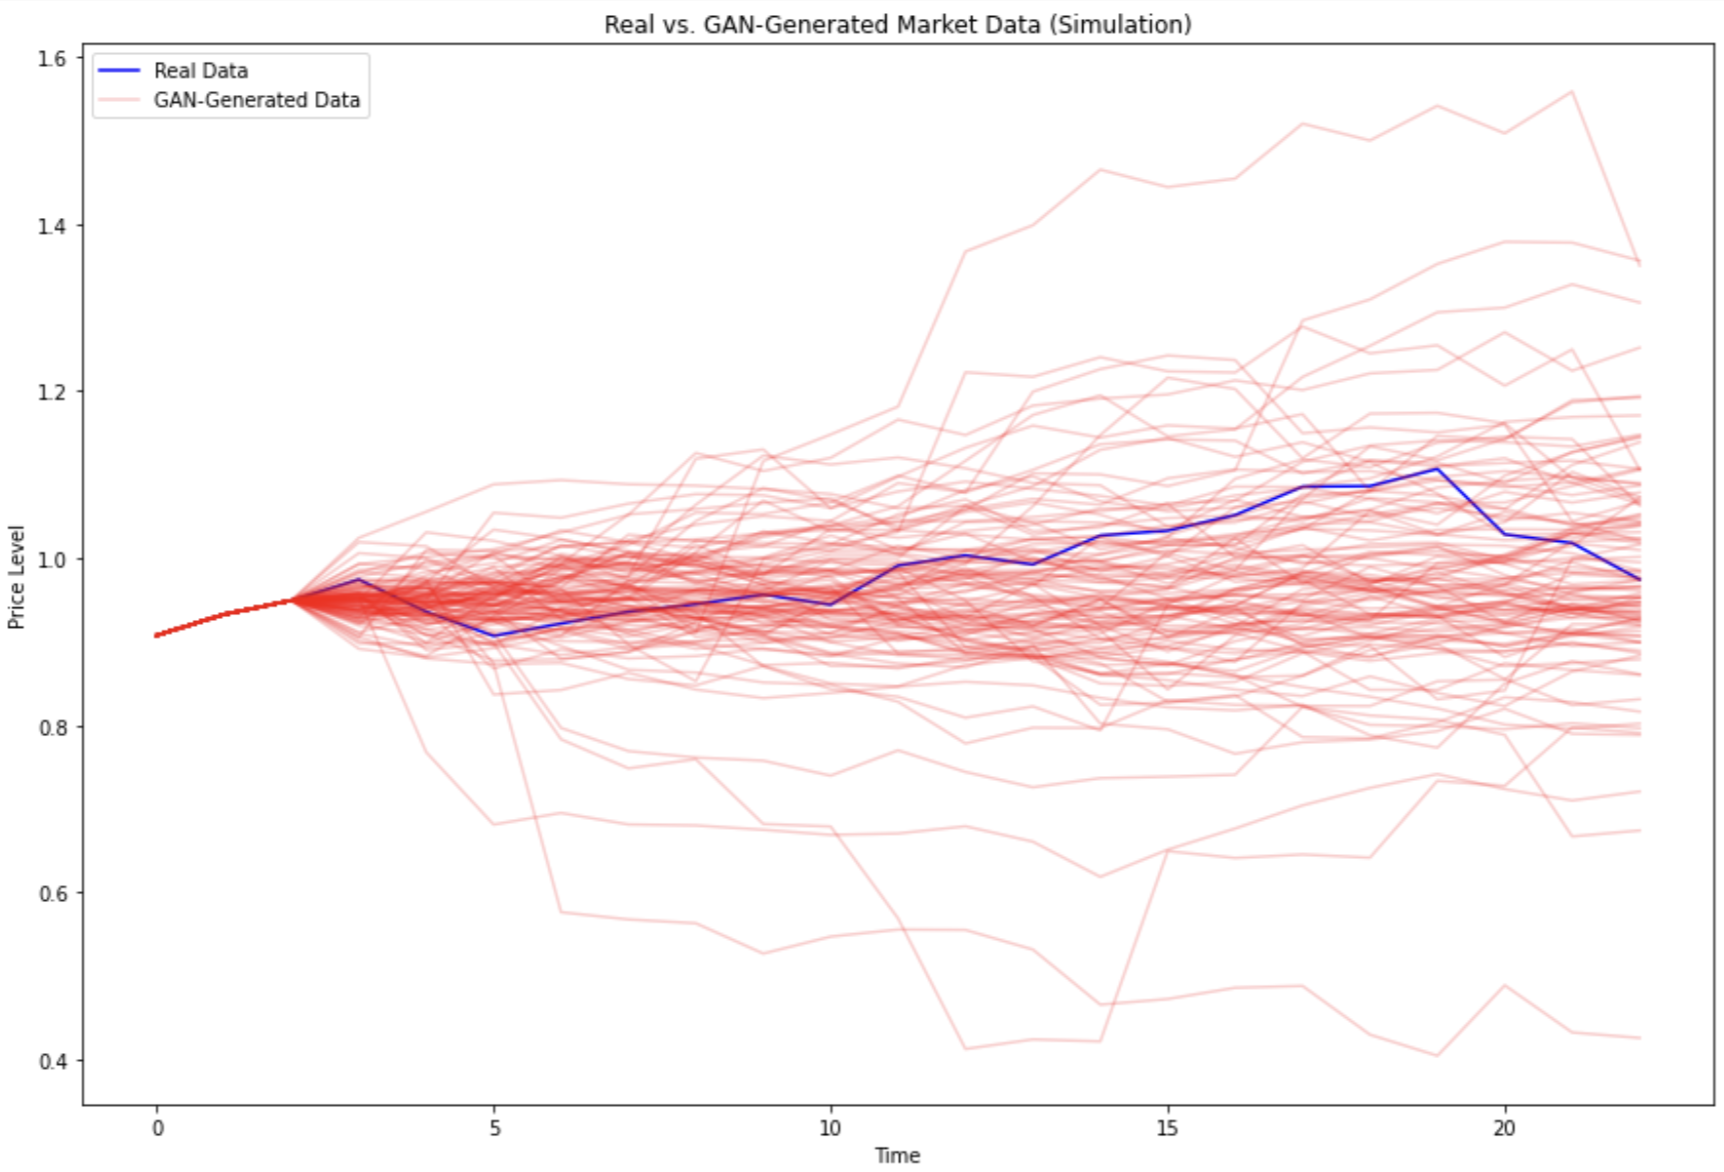
\includegraphics[width=14cm]{templates/assets/gan/gan_simulation.png}
\caption{GAN-Based Market Simulation of Price Paths}
\end{figure}

\section{Evaluating GAN-Based Market Simulations}
To be confident in the accuracy of GAN-generated market data in representing empirical data, there must be a systematic framework for quantitatively evaluating the similarity of synthetic data to real data. Unlike synthetic image generation with GANs, where the quality of the generated data can be visually observed by humans, synthetic time series and financial data are harder to evaluate directly. It is easier for humans to observe the facial features of generated images than it is to identify common-occurring statistical properties present in time series data.
\\
\\
However, since GANs are an unsupervised machine learning framework, there isn't a single or standard way to evaluate performance \cite{dh-simulating-equity}. With supervised machine learning methods, the standard way of measuring performance is to make predictions on a test data set and compute a metric such as accuracy or root mean square error. Since GANs are generating new data, it is infeasible to use the same evaluation methods. However, this does not mean that the similarity between GAN-generated synthetic data and real data cannot be measured. There are various metrics and statistics apparent in time-series data that can be measured, evaluated, and compared between synthetic market data and real market data. Ideally, these metrics will be similar in value which indicates that the GAN has learned the underlying distribution of the financial time-series data. Although it is difficult to explain GAN outputs, the metrics will bring confidence into the GAN learning market dynamics from data.

\subsection{Time-Series Distributional Statistics \& Metrics}

There are various time-series metrics and statistics that can be computed that describe the temporal dynamics and conditional distribution of the time-series data. For example, distributional statistics such as mean, median, minimum, and maximum may be useful for comparing real and synthetic data to ensure the synthetic data has a relatively similar distribution. There should be some degree of variation in the statistics so that the GAN is able to generate a diverse set of data.
\\
However, properties that exist in financial time-series data are often more complex in nature. It is simple to generate data with similar distributional statistics, as Monte Carlo methods do well, but difficult to mimic the exact temporal features that exist in financial data, since the exact properties of stock returns are unknown. To quantitatively evaluate the ability of the GAN to generate meaningful representations of market data, time-series feature extraction can be used. Maximilian Christ et al. (2018) explore various time-series feature extraction \cite{tsfresh} methods to gain insight into the temporal dynamics of time-series data. The \textbf{tsfresh} package encapsulates over 794 time-series features that can be used to describe the properties and behaviors of time-series data. A comprehensive list of all extracted features can be found on the official \textbf{tsfresh} documentation page. A summary of the time-series metrics is displayed below for real market data, GAN-generated data, and Monte Carlo simulations.
\begin{table}[h]
\begin{centering}
\begin{tabular}{@{\extracolsep{2pt}}lcccccc}
\toprule
Statistics & Mean   & Median   & Variance & Skewness & Kurtosis \\ \midrule
Real Market Data &   20.45          &   19.86       &     1.64      &      0.61        &      -0.96          \\
GAN Market Data        &     20.78        &    20.04      &     2.28      &       0.26       &    -1.66      \\
Monte Carlo Simulation & 22.37 & 21.49 & 1.32 & 0.21 & -0.25\\
\bottomrule
\end{tabular}
\caption{Distributional Statistics of Real vs. Synthetic Market Data}
\end{centering}
\end{table}

\begin{table}[h]
\begin{centering}
\begin{tabular}{@{\extracolsep{2pt}}lcccccc}
\toprule
Autocorrelation & Lag 1  & Lag 2  & Lag 3 & Lag 4 & Lag 5 \\ \midrule
Real Market Data &   0.84          &   0.72       &     0.61      &      0.47        &    0.36          \\
GAN Market Data        &     0.95        &    0.86      &     0.75      &       0.66       &    0.52  \\
Monte Carlo Simulation & 0.67 & 0.42 & 0.35 & 0.21 & 0.15\\
\bottomrule
\end{tabular}
\caption{Autocorrelation of Real vs. Synthetic Market Data}
\end{centering}
\end{table}

\noindent As shown from the distributional statistics and autocorrelations of the real and GAN-generated market data above, they appear to have similar properties. GAN-generated market data seems to emulate the patterns of real market data more closely than Monte Carlo simulations. This implies that there may be some specific properties or dynamics of stock price movement that are unable to be modeled by simple probabilistic simulations. These results demonstrate the efficacy of using GANs to generate representative market data that may be useful for other purposes.

\subsection{t-SNE Comparison}
There are a large number of tsfresh time-series features to compare manually. One method to evaluate how similar the metrics of the generator's synthetic data are to the empirical data is to use the t-distributed stochastic neighbor embedding (t-SNE) \cite{tsne} algorithm. As high-dimensional data is difficult to visualize, the t-SNE method visualizes the high-dimensional inputs by mapping the data from a high dimension to a low dimension. Using this method, we can compare the t-SNE mapping visualizations between the time-series metrics of generated market data and real market data. Using the generator to generate 1000 samples, the t-SNE plot of real (teal) and synthetic (red) financial time-series data metrics is displayed below.
\begin{figure}[h]
\centering
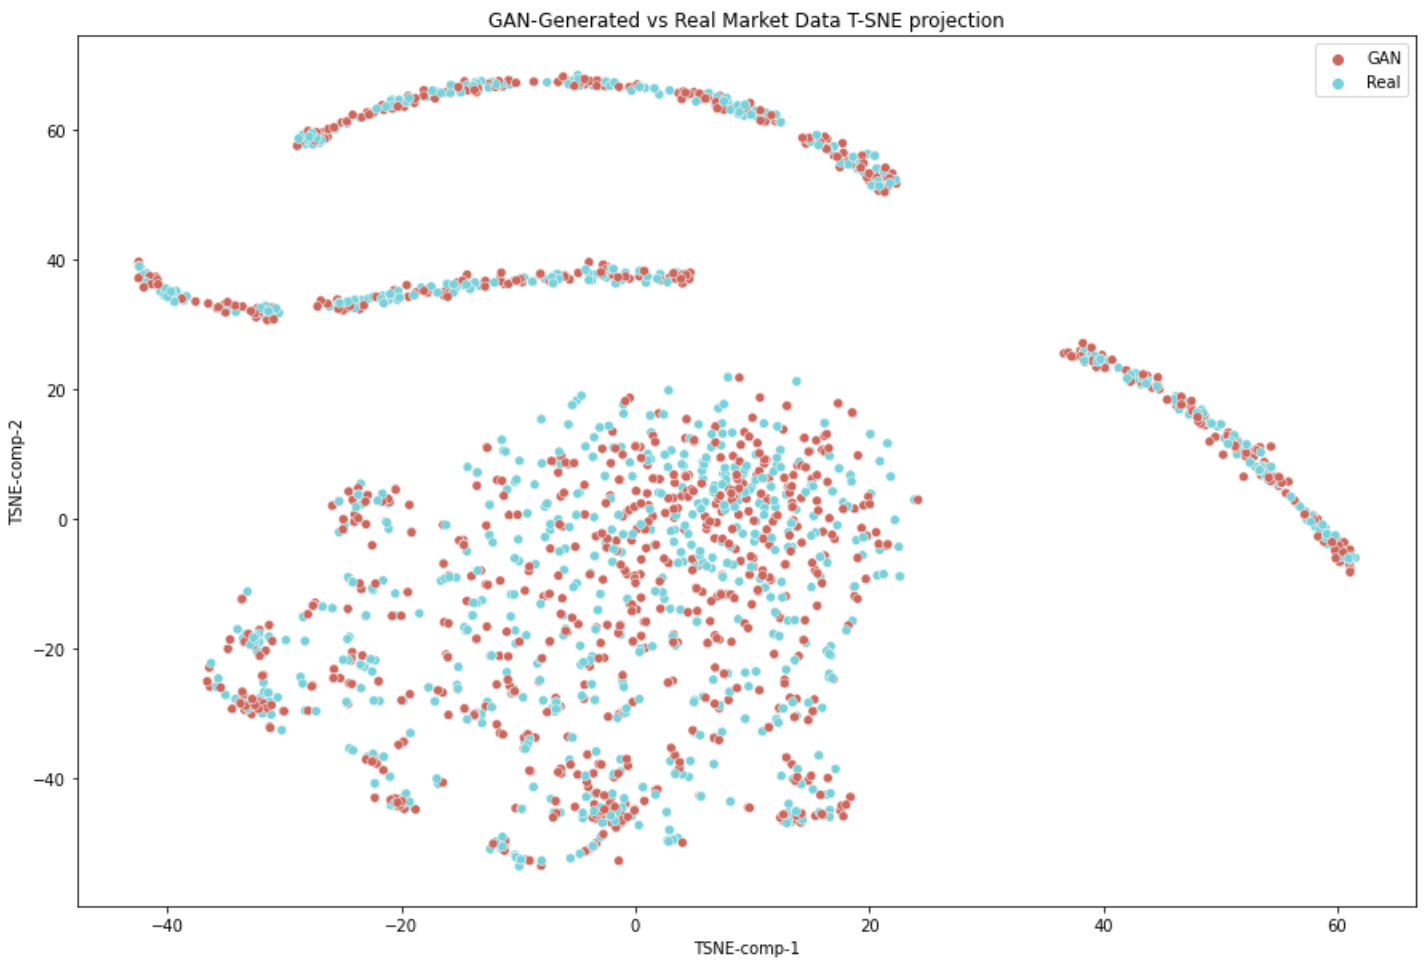
\includegraphics[width=14cm]{templates/assets/gan/tsne.png}
\caption{t-SNE Visualization of Real vs. Synthetic Market Data}
\end{figure}

\noindent The t-SNE visualization shows that the high-to-low dimensional mapping of the real data closely follows that of the GAN-generated data. This shows that the time-series features previously described are similar for both real and synthetic data, implying the GAN's ability to learn the properties of empirical stock returns. Being able to model complex market dynamics has great potential as will be explored in later chapters.
